%%%%%%%%%%%%%%%%%%%%%%%%%%%%%%%%%%%%%%%%%%%%%%%%%%%%%%%%%%%%%%%%%
%  _____       ______   ____									%
% |_   _|     |  ____|/ ____|  Institute of Embedded Systems	%
%   | |  _ __ | |__  | (___    Wireless Group					%
%   | | | '_ \|  __|  \___ \   Zuercher Hochschule Winterthur	%
%  _| |_| | | | |____ ____) |  (University of Applied Sciences)	%
% |_____|_| |_|______|_____/   8401 Winterthur, Switzerland		%
%																%
%%%%%%%%%%%%%%%%%%%%%%%%%%%%%%%%%%%%%%%%%%%%%%%%%%%%%%%%%%%%%%%%%


\pagenumbering{Roman}

\appendix






\section{Offizielle Aufgabenstellung}\label{sect.verzeichnis_literatur}
Projektauftrag

\section{CD mit vollständigem Bericht}\label{sect.verzeichnis_literatur}


\chapter{Anhang: Top Synthesizer}\label{chap.anhang_top_synthesizer}

In die bestehenden Blöcke und Signale wird das MIDI Interface wiefolgt eingebaut:\\
\begin{figure}[H]
	\centering
	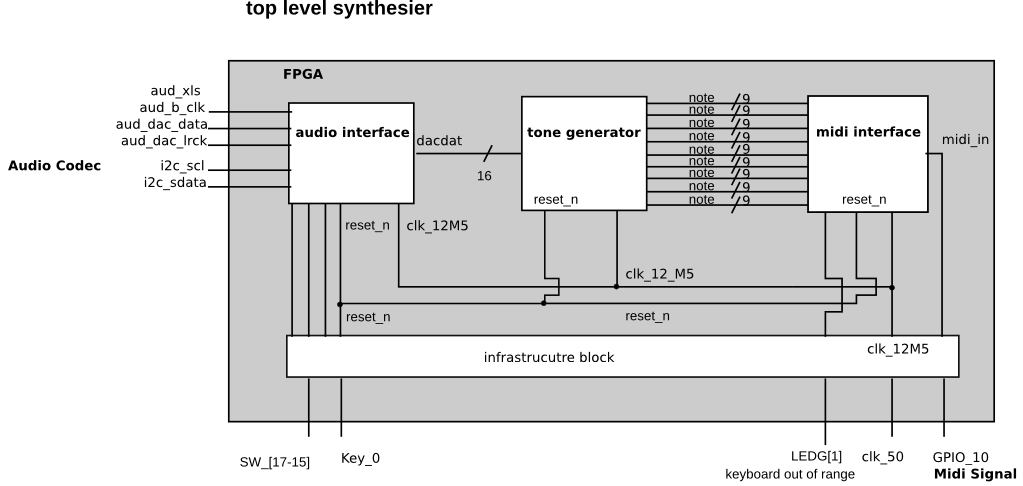
\includegraphics[width=1\textwidth]{images/midi_interface/top_synthesizer_block.png}
	\caption{Top Synthesizer mit MIDI Interface: Blockschaltbild}
	\label{fig.top_synthesizer_block}
\end{figure}

Hier ist das Konzept der Umsetzung des MIDI Interface detaillierter beschrieben:\\
\begin{figure}[H]
	\centering
	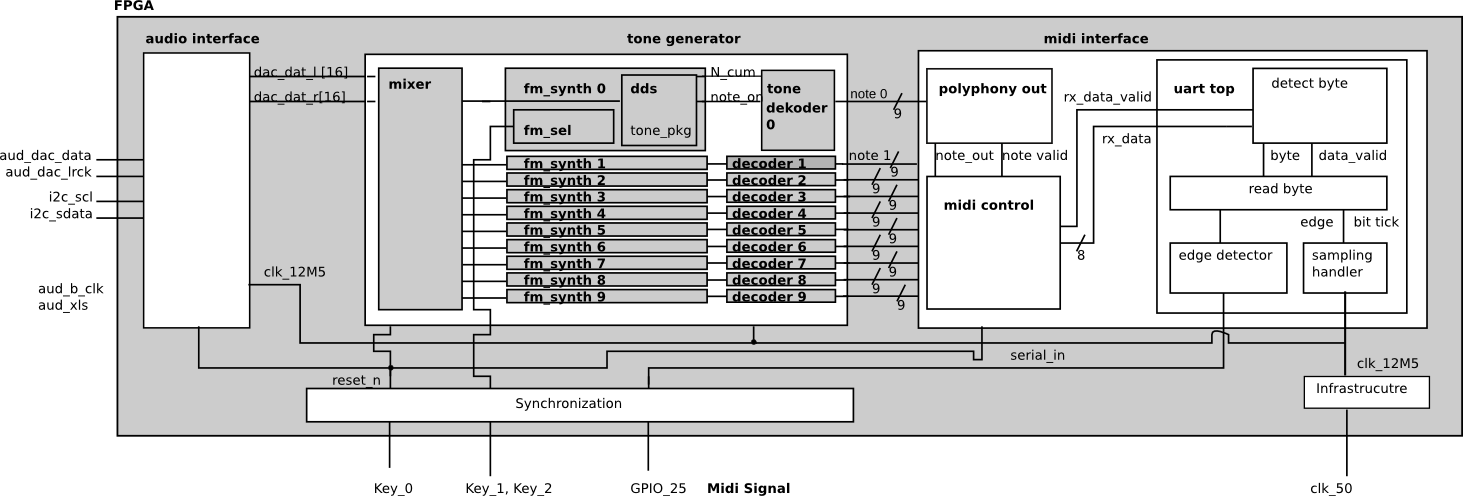
\includegraphics[width=1\textwidth]{images/midi_interface/top_synthesizer_detail.png}
	\caption{Top Synthesizer mit MIDI Interface: Detailansicht}
	\label{fig.top_synthesizer_detail}
\end{figure}




